% Options for packages loaded elsewhere
\PassOptionsToPackage{unicode}{hyperref}
\PassOptionsToPackage{hyphens}{url}
\PassOptionsToPackage{dvipsnames,svgnames,x11names}{xcolor}
%
\documentclass[
  letterpaper,
  DIV=11,
  numbers=noendperiod]{scrreprt}

\usepackage{amsmath,amssymb}
\usepackage{lmodern}
\usepackage{iftex}
\ifPDFTeX
  \usepackage[T1]{fontenc}
  \usepackage[utf8]{inputenc}
  \usepackage{textcomp} % provide euro and other symbols
\else % if luatex or xetex
  \usepackage{unicode-math}
  \defaultfontfeatures{Scale=MatchLowercase}
  \defaultfontfeatures[\rmfamily]{Ligatures=TeX,Scale=1}
\fi
% Use upquote if available, for straight quotes in verbatim environments
\IfFileExists{upquote.sty}{\usepackage{upquote}}{}
\IfFileExists{microtype.sty}{% use microtype if available
  \usepackage[]{microtype}
  \UseMicrotypeSet[protrusion]{basicmath} % disable protrusion for tt fonts
}{}
\makeatletter
\@ifundefined{KOMAClassName}{% if non-KOMA class
  \IfFileExists{parskip.sty}{%
    \usepackage{parskip}
  }{% else
    \setlength{\parindent}{0pt}
    \setlength{\parskip}{6pt plus 2pt minus 1pt}}
}{% if KOMA class
  \KOMAoptions{parskip=half}}
\makeatother
\usepackage{xcolor}
\setlength{\emergencystretch}{3em} % prevent overfull lines
\setcounter{secnumdepth}{-\maxdimen} % remove section numbering
% Make \paragraph and \subparagraph free-standing
\ifx\paragraph\undefined\else
  \let\oldparagraph\paragraph
  \renewcommand{\paragraph}[1]{\oldparagraph{#1}\mbox{}}
\fi
\ifx\subparagraph\undefined\else
  \let\oldsubparagraph\subparagraph
  \renewcommand{\subparagraph}[1]{\oldsubparagraph{#1}\mbox{}}
\fi

\usepackage{color}
\usepackage{fancyvrb}
\newcommand{\VerbBar}{|}
\newcommand{\VERB}{\Verb[commandchars=\\\{\}]}
\DefineVerbatimEnvironment{Highlighting}{Verbatim}{commandchars=\\\{\}}
% Add ',fontsize=\small' for more characters per line
\usepackage{framed}
\definecolor{shadecolor}{RGB}{241,243,245}
\newenvironment{Shaded}{\begin{snugshade}}{\end{snugshade}}
\newcommand{\AlertTok}[1]{\textcolor[rgb]{0.68,0.00,0.00}{#1}}
\newcommand{\AnnotationTok}[1]{\textcolor[rgb]{0.37,0.37,0.37}{#1}}
\newcommand{\AttributeTok}[1]{\textcolor[rgb]{0.40,0.45,0.13}{#1}}
\newcommand{\BaseNTok}[1]{\textcolor[rgb]{0.68,0.00,0.00}{#1}}
\newcommand{\BuiltInTok}[1]{\textcolor[rgb]{0.00,0.23,0.31}{#1}}
\newcommand{\CharTok}[1]{\textcolor[rgb]{0.13,0.47,0.30}{#1}}
\newcommand{\CommentTok}[1]{\textcolor[rgb]{0.37,0.37,0.37}{#1}}
\newcommand{\CommentVarTok}[1]{\textcolor[rgb]{0.37,0.37,0.37}{\textit{#1}}}
\newcommand{\ConstantTok}[1]{\textcolor[rgb]{0.56,0.35,0.01}{#1}}
\newcommand{\ControlFlowTok}[1]{\textcolor[rgb]{0.00,0.23,0.31}{#1}}
\newcommand{\DataTypeTok}[1]{\textcolor[rgb]{0.68,0.00,0.00}{#1}}
\newcommand{\DecValTok}[1]{\textcolor[rgb]{0.68,0.00,0.00}{#1}}
\newcommand{\DocumentationTok}[1]{\textcolor[rgb]{0.37,0.37,0.37}{\textit{#1}}}
\newcommand{\ErrorTok}[1]{\textcolor[rgb]{0.68,0.00,0.00}{#1}}
\newcommand{\ExtensionTok}[1]{\textcolor[rgb]{0.00,0.23,0.31}{#1}}
\newcommand{\FloatTok}[1]{\textcolor[rgb]{0.68,0.00,0.00}{#1}}
\newcommand{\FunctionTok}[1]{\textcolor[rgb]{0.28,0.35,0.67}{#1}}
\newcommand{\ImportTok}[1]{\textcolor[rgb]{0.00,0.46,0.62}{#1}}
\newcommand{\InformationTok}[1]{\textcolor[rgb]{0.37,0.37,0.37}{#1}}
\newcommand{\KeywordTok}[1]{\textcolor[rgb]{0.00,0.23,0.31}{#1}}
\newcommand{\NormalTok}[1]{\textcolor[rgb]{0.00,0.23,0.31}{#1}}
\newcommand{\OperatorTok}[1]{\textcolor[rgb]{0.37,0.37,0.37}{#1}}
\newcommand{\OtherTok}[1]{\textcolor[rgb]{0.00,0.23,0.31}{#1}}
\newcommand{\PreprocessorTok}[1]{\textcolor[rgb]{0.68,0.00,0.00}{#1}}
\newcommand{\RegionMarkerTok}[1]{\textcolor[rgb]{0.00,0.23,0.31}{#1}}
\newcommand{\SpecialCharTok}[1]{\textcolor[rgb]{0.37,0.37,0.37}{#1}}
\newcommand{\SpecialStringTok}[1]{\textcolor[rgb]{0.13,0.47,0.30}{#1}}
\newcommand{\StringTok}[1]{\textcolor[rgb]{0.13,0.47,0.30}{#1}}
\newcommand{\VariableTok}[1]{\textcolor[rgb]{0.07,0.07,0.07}{#1}}
\newcommand{\VerbatimStringTok}[1]{\textcolor[rgb]{0.13,0.47,0.30}{#1}}
\newcommand{\WarningTok}[1]{\textcolor[rgb]{0.37,0.37,0.37}{\textit{#1}}}

\providecommand{\tightlist}{%
  \setlength{\itemsep}{0pt}\setlength{\parskip}{0pt}}\usepackage{longtable,booktabs,array}
\usepackage{calc} % for calculating minipage widths
% Correct order of tables after \paragraph or \subparagraph
\usepackage{etoolbox}
\makeatletter
\patchcmd\longtable{\par}{\if@noskipsec\mbox{}\fi\par}{}{}
\makeatother
% Allow footnotes in longtable head/foot
\IfFileExists{footnotehyper.sty}{\usepackage{footnotehyper}}{\usepackage{footnote}}
\makesavenoteenv{longtable}
\usepackage{graphicx}
\makeatletter
\def\maxwidth{\ifdim\Gin@nat@width>\linewidth\linewidth\else\Gin@nat@width\fi}
\def\maxheight{\ifdim\Gin@nat@height>\textheight\textheight\else\Gin@nat@height\fi}
\makeatother
% Scale images if necessary, so that they will not overflow the page
% margins by default, and it is still possible to overwrite the defaults
% using explicit options in \includegraphics[width, height, ...]{}
\setkeys{Gin}{width=\maxwidth,height=\maxheight,keepaspectratio}
% Set default figure placement to htbp
\makeatletter
\def\fps@figure{htbp}
\makeatother

\KOMAoption{captions}{tableheading}
\makeatletter
\makeatother
\makeatletter
\makeatother
\makeatletter
\@ifpackageloaded{caption}{}{\usepackage{caption}}
\AtBeginDocument{%
\ifdefined\contentsname
  \renewcommand*\contentsname{Table of contents}
\else
  \newcommand\contentsname{Table of contents}
\fi
\ifdefined\listfigurename
  \renewcommand*\listfigurename{List of Figures}
\else
  \newcommand\listfigurename{List of Figures}
\fi
\ifdefined\listtablename
  \renewcommand*\listtablename{List of Tables}
\else
  \newcommand\listtablename{List of Tables}
\fi
\ifdefined\figurename
  \renewcommand*\figurename{Figure}
\else
  \newcommand\figurename{Figure}
\fi
\ifdefined\tablename
  \renewcommand*\tablename{Table}
\else
  \newcommand\tablename{Table}
\fi
}
\@ifpackageloaded{float}{}{\usepackage{float}}
\floatstyle{ruled}
\@ifundefined{c@chapter}{\newfloat{codelisting}{h}{lop}}{\newfloat{codelisting}{h}{lop}[chapter]}
\floatname{codelisting}{Listing}
\newcommand*\listoflistings{\listof{codelisting}{List of Listings}}
\makeatother
\makeatletter
\@ifpackageloaded{caption}{}{\usepackage{caption}}
\@ifpackageloaded{subcaption}{}{\usepackage{subcaption}}
\makeatother
\makeatletter
\@ifpackageloaded{tcolorbox}{}{\usepackage[many]{tcolorbox}}
\makeatother
\makeatletter
\@ifundefined{shadecolor}{\definecolor{shadecolor}{rgb}{.97, .97, .97}}
\makeatother
\makeatletter
\makeatother
\ifLuaTeX
  \usepackage{selnolig}  % disable illegal ligatures
\fi
\IfFileExists{bookmark.sty}{\usepackage{bookmark}}{\usepackage{hyperref}}
\IfFileExists{xurl.sty}{\usepackage{xurl}}{} % add URL line breaks if available
\urlstyle{same} % disable monospaced font for URLs
\hypersetup{
  colorlinks=true,
  linkcolor={blue},
  filecolor={Maroon},
  citecolor={Blue},
  urlcolor={Blue},
  pdfcreator={LaTeX via pandoc}}

\author{}
\date{}

\begin{document}
\ifdefined\Shaded\renewenvironment{Shaded}{\begin{tcolorbox}[breakable, boxrule=0pt, interior hidden, borderline west={3pt}{0pt}{shadecolor}, enhanced, sharp corners, frame hidden]}{\end{tcolorbox}}\fi

\hypertarget{spatiotemporal-data}{%
\chapter{Spatiotemporal Data}\label{spatiotemporal-data}}

\hypertarget{workshop-3-open-in-colab}{%
\section[\emph{Workshop 3} ]{\texorpdfstring{\emph{Workshop 3}
\href{https://colab.research.google.com/github/oballinger/QM2/blob/main/notebooks/W03.\%20Spatial\%20Data.ipynb}{\protect
\includegraphics{https://github.com/oballinger/QM2/blob/main/colab-badge.png?raw=1}}}{Workshop 3 Open In Colab}}\label{workshop-3-open-in-colab}}

Sometimes the data we work with references points on the earth's
surface, unlocking a rich set of analytical possibilities. In today's
workshop, we're going to be exploring the effect of the 2020 California
Wildfires on air quality across the state. We'll be using real air
quality data collected by sensors and combining it with satellite
imagery to show how toxic smoke from wildfires swept over America's
largest state.

\hypertarget{aims}{%
\subsection{Aims}\label{aims}}

\begin{itemize}
\tightlist
\item
  Understanding spatiotemporal data
\item
  Grouping data in pandas
\item
  Manipulating and plotting geographic data
\end{itemize}

\hypertarget{background}{%
\section{Background}\label{background}}

\includegraphics{https://image.cnbcfm.com/api/v1/image/106695701-1599664926959-gettyimages-1228423382-AFP_8PL8JF.jpeg?v=1599664969}

The \href{https://en.wikipedia.org/wiki/2020_California_wildfires}{2020
California wildfire season} was record-setting. By the end of the year,
9,917 fires had burned more than 4\% of the state's area, making 2020
the largest wildfire season recorded in California's modern history.
California's August Complex fire has been described as the first
``gigafire'', burning over 1 million acres across seven counties, an
area larger than the state of Rhode Island. The fires destroyed over
10,000 structures and cost over \$12.079 billion (2020 USD) in damages,
including over \$10 billion in property damage and \$2.079 billion in
fire suppression costs. The intensity of the fire season has been
attributed to a combination of more than a century of poor forest
management and higher temperatures resulting from climate change.

The fires also had a
\href{https://epic.uchicago.edu/news/pollution-from-californias-2020-wildfires-likely-offset-decades-of-air-quality-gains/}{profound
effect on air quality}: ``Places that are experiencing frequent or more
frequent wildfires are going to experience higher air pollution levels,
not just for a couple of days or weeks, but it could impact the annual
level of exposure,'' said Christa Hasenkopf, director of air quality
programs at the University of Chicago institute. ``It can bump up that
average to unsafe and unhealthy levels that really do have an impact on
people's health. When we think of wildfires, we think of short-term
events --- and hopefully they are --- but they can have long-term
consequences considering your overall air pollution exposure.''

\hypertarget{getting-started}{%
\section{Getting Started}\label{getting-started}}

Let's begin by installing some libraries that we'll be working with
today.

\begin{Shaded}
\begin{Highlighting}[]
\OperatorTok{\%\%}\NormalTok{capture}
\OperatorTok{!}\NormalTok{pip install Basemap}
\OperatorTok{!}\NormalTok{pip install ipyleaflet}
\end{Highlighting}
\end{Shaded}

\hypertarget{importing-libraries}{%
\section{Importing Libraries}\label{importing-libraries}}

The first step in any python script is to import the necessary
libraries:

\begin{Shaded}
\begin{Highlighting}[]
\ImportTok{import}\NormalTok{ pandas }\ImportTok{as}\NormalTok{ pd}
\ImportTok{import}\NormalTok{ matplotlib}
\ImportTok{import}\NormalTok{ matplotlib.pyplot }\ImportTok{as}\NormalTok{ plt}
\ImportTok{import}\NormalTok{ numpy }\ImportTok{as}\NormalTok{ np}
\ImportTok{import}\NormalTok{ pylab}
\ImportTok{from}\NormalTok{ datetime }\ImportTok{import}\NormalTok{ datetime}

\OperatorTok{\%}\NormalTok{matplotlib inline}
\NormalTok{pylab.rcParams[}\StringTok{\textquotesingle{}figure.figsize\textquotesingle{}}\NormalTok{] }\OperatorTok{=}\NormalTok{ (}\DecValTok{10}\NormalTok{, }\DecValTok{8}\NormalTok{)}
\end{Highlighting}
\end{Shaded}

\hypertarget{downloading-data}{%
\section{Downloading Data}\label{downloading-data}}

The next step is to import the data that we need for our analysis. This
week we'll be using real data collected in 2020 by the
\href{https://www.epa.gov/outdoor-air-quality-data/download-daily-data}{Environmental
Protection Agency (EPA)}. I've generated a .csv file containing the data
that I want using the dropdown menus. The EPA also has an
\href{https://aqs.epa.gov/aqsweb/documents/data_api.html}{Application
Programming Interface} for air quality data, which you could use to pull
in data directly into python without having to download a .csv!

\begin{Shaded}
\begin{Highlighting}[]
\OperatorTok{!}\NormalTok{mkdir data}
\OperatorTok{!}\NormalTok{mkdir data}\OperatorTok{/}\NormalTok{wk3}
\OperatorTok{!}\NormalTok{curl https:}\OperatorTok{//}\NormalTok{qm2.s3.eu}\OperatorTok{{-}}\NormalTok{west}\OperatorTok{{-}}\FloatTok{2.}\ErrorTok{amazonaws}\NormalTok{.com}\OperatorTok{/}\NormalTok{wk3}\OperatorTok{/}\NormalTok{california\_aqi.csv }\OperatorTok{{-}}\NormalTok{o .}\OperatorTok{/}\NormalTok{data}\OperatorTok{/}\NormalTok{wk3}\OperatorTok{/}\NormalTok{california\_aqi.csv}
\end{Highlighting}
\end{Shaded}

\begin{verbatim}
  % Total    % Received % Xferd  Average Speed   Time    Time     Time  Current
                                 Dload  Upload   Total   Spent    Left  Speed
100 5586k  100 5586k    0     0  4476k      0  0:00:01  0:00:01 --:--:-- 4479k
\end{verbatim}

Let's open the .csv file and have a look at it:

\begin{Shaded}
\begin{Highlighting}[]
\NormalTok{df}\OperatorTok{=}\NormalTok{pd.read\_csv(}\StringTok{\textquotesingle{}data/wk3/california\_aqi.csv\textquotesingle{}}\NormalTok{)}
\NormalTok{df}
\end{Highlighting}
\end{Shaded}

\begin{longtable}[]{@{}lllllllllll@{}}
\toprule()
& Date & Site ID & POC & PM & AQI & Site Name & CBSA\_NAME & COUNTY &
latitude & longitude \\
\midrule()
\endhead
0 & 1/1/20 & 60010007 & 3 & 8.6 & 36 & Livermore & San
Francisco-Oakland-Hayward, CA & Alameda & 37.687526 & -121.784217 \\
1 & 1/2/20 & 60010007 & 3 & 4.5 & 19 & Livermore & San
Francisco-Oakland-Hayward, CA & Alameda & 37.687526 & -121.784217 \\
2 & 1/3/20 & 60010007 & 3 & 14.2 & 55 & Livermore & San
Francisco-Oakland-Hayward, CA & Alameda & 37.687526 & -121.784217 \\
3 & 1/4/20 & 60010007 & 3 & 10.9 & 45 & Livermore & San
Francisco-Oakland-Hayward, CA & Alameda & 37.687526 & -121.784217 \\
4 & 1/5/20 & 60010007 & 3 & 7.8 & 33 & Livermore & San
Francisco-Oakland-Hayward, CA & Alameda & 37.687526 & -121.784217 \\
... & ... & ... & ... & ... & ... & ... & ... & ... & ... & ... \\
55686 & 11/29/20 & 61131003 & 1 & 20.3 & 68 & Woodland-Gibson Road &
Sacramento-\/-Roseville-\/-Arden-Arcade, CA & Yolo & 38.661210 &
-121.732690 \\
55687 & 12/18/20 & 61131003 & 1 & 2.8 & 12 & Woodland-Gibson Road &
Sacramento-\/-Roseville-\/-Arden-Arcade, CA & Yolo & 38.661210 &
-121.732690 \\
55688 & 12/20/20 & 61131003 & 1 & 22.4 & 73 & Woodland-Gibson Road &
Sacramento-\/-Roseville-\/-Arden-Arcade, CA & Yolo & 38.661210 &
-121.732690 \\
55689 & 12/23/20 & 61131003 & 1 & 11.8 & 49 & Woodland-Gibson Road &
Sacramento-\/-Roseville-\/-Arden-Arcade, CA & Yolo & 38.661210 &
-121.732690 \\
55690 & 12/29/20 & 61131003 & 1 & 5.6 & 23 & Woodland-Gibson Road &
Sacramento-\/-Roseville-\/-Arden-Arcade, CA & Yolo & 38.661210 &
-121.732690 \\
\bottomrule()
\end{longtable}

Each row in this dataset is an individual reading from an air quality
sensor. The first row is a reading from sensor number 60010007 on
January 1st 2020. It is located in Alameda County, and recorded an Air
Quality Index (AQI) reading of 36. So for each sensor (uniquely
identified by the Site ID column) we will have 365 readings. We also
have the latitude and longitude of each one of these air quality
sensors. The presence of these fields makes this
\textbf{spatio-temporal} data. We'll first analyze the temporal
dimension of our data, before adding in the spatial dimension

\hypertarget{temporal-data}{%
\section{Temporal Data}\label{temporal-data}}

Before we go any further, we need to focus on a very special column in
our dataset: the ``Date'' column. We'll be relying heavily on this
dimension of our dataset. Whenever we have temporal data, the first
thing we want to do is check whether pandas is storing it as datetime
information or as a string (text). We can do this using the
\texttt{dtype} function.

\begin{Shaded}
\begin{Highlighting}[]
\BuiltInTok{print}\NormalTok{(}\StringTok{\textquotesingle{}Prior to cleaning, the data type of the "Date" column is:\textquotesingle{}}\NormalTok{, df[}\StringTok{\textquotesingle{}Date\textquotesingle{}}\NormalTok{].dtype)}

\NormalTok{df[}\StringTok{\textquotesingle{}Date\textquotesingle{}}\NormalTok{]}\OperatorTok{=}\NormalTok{pd.to\_datetime(df[}\StringTok{\textquotesingle{}Date\textquotesingle{}}\NormalTok{])}

\BuiltInTok{print}\NormalTok{(}\StringTok{\textquotesingle{}Now, it is stored as: \textquotesingle{}}\NormalTok{, df[}\StringTok{\textquotesingle{}Date\textquotesingle{}}\NormalTok{].dtype)}
\end{Highlighting}
\end{Shaded}

\begin{verbatim}
Prior to cleaning, the data type of the "Date" column is: object
Now, it is stored as:  datetime64[ns]
\end{verbatim}

Once we've stored the Date column as datetime information, we can do all
sorts of useful things with it. For example, we can quickly extract the
month from the date, or even the ``day of year'' (i.e., how many days
since January 1st of that year have passed). Try doing that in one line
of code if your ``Date'' column is stored as text!

\begin{Shaded}
\begin{Highlighting}[]
\CommentTok{\# we can extract the month from the Date column and save it as a new column }
\NormalTok{df[}\StringTok{\textquotesingle{}Month\textquotesingle{}}\NormalTok{]}\OperatorTok{=}\NormalTok{df[}\StringTok{\textquotesingle{}Date\textquotesingle{}}\NormalTok{].dt.month}
\CommentTok{\# we can do the same for the day of year. }
\NormalTok{df[}\StringTok{\textquotesingle{}Day\textquotesingle{}}\NormalTok{]}\OperatorTok{=}\NormalTok{df[}\StringTok{\textquotesingle{}Date\textquotesingle{}}\NormalTok{].dt.dayofyear}

\BuiltInTok{print}\NormalTok{(df[[}\StringTok{\textquotesingle{}Date\textquotesingle{}}\NormalTok{,}\StringTok{\textquotesingle{}Month\textquotesingle{}}\NormalTok{,}\StringTok{\textquotesingle{}Day\textquotesingle{}}\NormalTok{]])}
\end{Highlighting}
\end{Shaded}

\begin{verbatim}
            Date  Month  Day
0     2020-01-01      1    1
1     2020-01-02      1    2
2     2020-01-03      1    3
3     2020-01-04      1    4
4     2020-01-05      1    5
...          ...    ...  ...
55686 2020-11-29     11  334
55687 2020-12-18     12  353
55688 2020-12-20     12  355
55689 2020-12-23     12  358
55690 2020-12-29     12  364

[55691 rows x 3 columns]
\end{verbatim}

When I print the new columns we've made (``Month'' and ``Day'') next to
the original ``Date'' column, we can see that everything is working as
it should. First date (January 1st, 2020), has a value of 1 in the month
column, and a 1 in the day column. The last row in the dataset was a
sensor reading raken on December 29th, 2020. It has a month of 12, and
day-of-year value of 364. Great.

\hypertarget{exercise}{%
\subsection{Exercise}\label{exercise}}

\href{https://pandas.pydata.org/docs/reference/api/pandas.Series.dt.dayofyear.html}{Here's}
the documentation for the pandas function that allowed us to extract the
day of year from the datetime column. Using the documentation on this
page, create a new column in the dataframe that contains the week of
year.

\hypertarget{grouping-data}{%
\subsection{Grouping Data}\label{grouping-data}}

We can now use the new temporal columns we've created to analyze our
data further. The broadest possible question we're interested in today
is ``What was the effect of the 2020 wildfires on air quality in
California?'' This involves looking at air quality over time, and
comparing pre/post wildfire air quality reading.

To translate that into python, we effectively want to calculate the
average AQI value for all of the sensors in California each day. We can
accomplish this using the \texttt{.groupby()} function in pandas.
\href{https://pandas.pydata.org/docs/reference/api/pandas.DataFrame.groupby.html}{Here}
is the documentation page for the function, give it a quick read.

Remember, each row in our dataframe \texttt{df} is an individual sensor
reading on a given day. We now want a dataframe in which each row is
\emph{one day}, representing the average of \emph{all AQI sensors}. We
can accomplish that using the following line of code, which has four
parts:

\texttt{df.groupby(\textquotesingle{}Day\textquotesingle{}){[}\textquotesingle{}AQI\textquotesingle{}{]}.mean()}

\begin{enumerate}
\def\labelenumi{\arabic{enumi}.}
\tightlist
\item
  \texttt{df}: the dataframe we want to use
\item
  \texttt{.groupby(\textquotesingle{}Day\textquotesingle{})}: the
  groupby function, and the name of the column that we want to group our
  data by. In this case, we want each row in our new dataset to be one
  day, so we're using the ``Day'' column.
\item
  \texttt{{[}\textquotesingle{}AQI\textquotesingle{}{]}}: the data that
  we want to aggregate. Remember, our dataframe has many columns, but we
  want to calculate the average daily value of AQI.
\item
  \texttt{.mean()}: the method of aggregation. We're calculating the
  average in this case, but we could also want to take the maximum value
  (\texttt{.max()}), minimum value (\texttt{.min()}), median
  (\texttt{.median()}), etc.
\end{enumerate}

Let's look at the output from the line of code above. Remember, whenever
we make something new, we must store it somewhere or it disappears! I'm
storing this as a new dataframe called ``daily''.

\begin{Shaded}
\begin{Highlighting}[]
\NormalTok{daily}\OperatorTok{=}\NormalTok{df.groupby(}\StringTok{\textquotesingle{}Day\textquotesingle{}}\NormalTok{)[}\StringTok{\textquotesingle{}AQI\textquotesingle{}}\NormalTok{].mean()}
\NormalTok{daily}
\end{Highlighting}
\end{Shaded}

\begin{verbatim}
Day
1      50.255682
2      43.300000
3      50.437500
4      47.224299
5      39.240602
         ...    
362    33.500000
363    23.358209
364    30.610256
365    39.492754
366    42.532374
Name: AQI, Length: 366, dtype: float64
\end{verbatim}

Now we can see that our dataframe has 366 rows, one for each day of the
year (2020 was actually a leap year!). Let's plot the daily average of
the AQI sensors, along with a dashed vertical line indicating the day a
State of Emergency was declared (August 18th).

\begin{Shaded}
\begin{Highlighting}[]
\CommentTok{\# plot the daily data}
\NormalTok{daily.plot(color}\OperatorTok{=}\StringTok{\textquotesingle{}red\textquotesingle{}}\NormalTok{)}

\CommentTok{\#add title and axis labels}
\NormalTok{plt.title(}\StringTok{\textquotesingle{}Daily Air Quality Index readings in California, 2020\textquotesingle{}}\NormalTok{)}
\NormalTok{plt.ylabel(}\StringTok{\textquotesingle{}AQI\textquotesingle{}}\NormalTok{)}
\NormalTok{plt.xlabel(}\StringTok{\textquotesingle{}Day of Year\textquotesingle{}}\NormalTok{)}

\CommentTok{\# add a dashed black line on August 18th (the 231st day of the year)}
\NormalTok{plt.axvline(}\DecValTok{231}\NormalTok{, color}\OperatorTok{=}\StringTok{\textquotesingle{}black\textquotesingle{}}\NormalTok{, linestyle}\OperatorTok{=}\StringTok{\textquotesingle{}{-}{-}\textquotesingle{}}\NormalTok{, label}\OperatorTok{=}\StringTok{\textquotesingle{}State of Emergency\textquotesingle{}}\NormalTok{)}
\NormalTok{plt.legend()}
\end{Highlighting}
\end{Shaded}

\begin{verbatim}
<matplotlib.legend.Legend at 0x7f6d0e2ab550>
\end{verbatim}

\begin{figure}[H]

{\centering 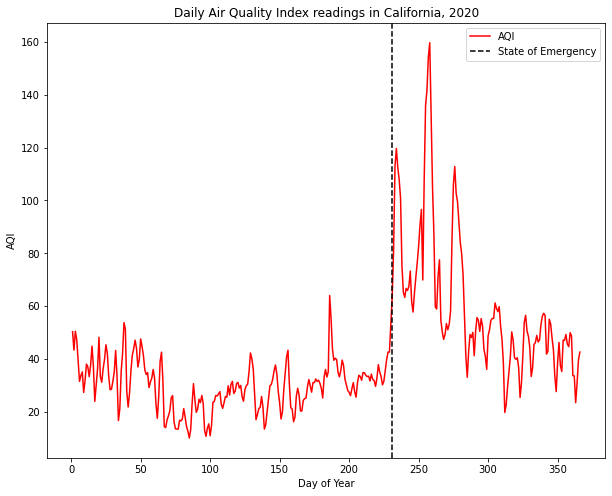
\includegraphics{W03. Spatial Data_files/figure-pdf/cell-10-output-2.png}

}

\end{figure}

Pretty cool! We can clearly see some spikes in AQI that correspond
directly to when the state of emergency was declared. Our data is
matching expectations about reality: even though there's no information
about the state of emergency or the wildfires in our dataframe
(remember, it's just a bunch of air quality readings from sensors), we
observe a relationship between our variables (presence of wildfires and
air quality) that conforms to our expectations.

\hypertarget{exercise-1}{%
\subsection{Exercise}\label{exercise-1}}

Now, repeat the above plot but aggregate the dataframe by month rather
than by day. Store the monthly data as a new dataframe called
``monthly''.

\hypertarget{geographic-disparities}{%
\subsection{Geographic Disparities}\label{geographic-disparities}}

OK. We've got a good sense of how the wildfires affected air quality
readings across the whole state. But California is huge; there are
probably geographic disparities in how bad air quality was as a result
of the fires. Let's see which counties were worst affected by the
wildfires.

In our original dataframe, each row was a reading from a given sensor on
a given day. We grouped this data by day to create a dataframe that took
the average of \emph{all} sensors in california for each day as follows:

\texttt{df.groupby(\textquotesingle{}Day\textquotesingle{}){[}\textquotesingle{}AQI\textquotesingle{}{]}.mean()}

Now, we want to plot the average daily air quality by county; this will
involve aggregating both by day \emph{and by county}. Intuitively, we
can accomplish this changing
\texttt{\textquotesingle{}Day\textquotesingle{}} to
\texttt{{[}\textquotesingle{}Day\textquotesingle{},\textquotesingle{}COUNTY\textquotesingle{}{]}},
like so:

\texttt{df.groupby({[}\textquotesingle{}Day\textquotesingle{},\textquotesingle{}COUNTY\textquotesingle{}{]}){[}\textquotesingle{}AQI\textquotesingle{}{]}.mean()}

Let's store this new dataframe and call it ``county\_daily'':

\begin{Shaded}
\begin{Highlighting}[]
\NormalTok{county\_daily}\OperatorTok{=}\NormalTok{df.groupby([}\StringTok{\textquotesingle{}Day\textquotesingle{}}\NormalTok{,}\StringTok{\textquotesingle{}COUNTY\textquotesingle{}}\NormalTok{,])[}\StringTok{\textquotesingle{}AQI\textquotesingle{}}\NormalTok{].mean().reset\_index()}
\NormalTok{county\_daily}
\end{Highlighting}
\end{Shaded}

\begin{longtable}[]{@{}llll@{}}
\toprule()
& Day & COUNTY & AQI \\
\midrule()
\endhead
0 & 1 & Alameda & 44.500000 \\
1 & 1 & Butte & 66.666667 \\
2 & 1 & Calaveras & 63.000000 \\
3 & 1 & Colusa & 78.000000 \\
4 & 1 & Contra Costa & 46.000000 \\
... & ... & ... & ... \\
17314 & 366 & Tehama & 52.000000 \\
17315 & 366 & Trinity & 36.000000 \\
17316 & 366 & Tulare & 62.666667 \\
17317 & 366 & Ventura & 23.666667 \\
17318 & 366 & Yolo & 35.000000 \\
\bottomrule()
\end{longtable}

\hypertarget{exercise-2}{%
\section{Exercise}\label{exercise-2}}

Using the \texttt{groupby} function, create a new dataframe called
``counties'' in which each row is a county, and each value is the
\textbf{maximum} AQI value in that county during the entire year. Then,
sort this dataframe in descending order using
\texttt{.sort\_values(ascending=False)}

Which county had the highest maximum AQI value? Which county had the
lowest? store the names of these counties as varables called ``highest''
and ``lowest'', shown below:

\begin{Shaded}
\begin{Highlighting}[]
\NormalTok{highest}\OperatorTok{=}\StringTok{\textquotesingle{}\textquotesingle{}}
\NormalTok{lowest}\OperatorTok{=}\StringTok{\textquotesingle{}\textquotesingle{}}

\CommentTok{\# Filter the county{-}level daily AQI readings for the worst{-}affected county}
\NormalTok{worst\_county}\OperatorTok{=}\NormalTok{county\_daily[county\_daily[}\StringTok{\textquotesingle{}COUNTY\textquotesingle{}}\NormalTok{]}\OperatorTok{==}\NormalTok{highest]}

\CommentTok{\# Filter the county{-}level daily AQI readings for the least{-}affected county}
\NormalTok{best\_county}\OperatorTok{=}\NormalTok{county\_daily[county\_daily[}\StringTok{\textquotesingle{}COUNTY\textquotesingle{}}\NormalTok{]}\OperatorTok{==}\NormalTok{lowest]}
\end{Highlighting}
\end{Shaded}

Using those two variables, lets plot the AQI values for each of these
counties individually:

\begin{Shaded}
\begin{Highlighting}[]
\CommentTok{\# plot the data from the worst affected county}
\NormalTok{plt.plot(worst\_county[}\StringTok{\textquotesingle{}Day\textquotesingle{}}\NormalTok{], worst\_county[}\StringTok{\textquotesingle{}AQI\textquotesingle{}}\NormalTok{], label}\OperatorTok{=}\NormalTok{highest)}

\CommentTok{\# plot the data from the least affected county}
\NormalTok{plt.plot(best\_county[}\StringTok{\textquotesingle{}Day\textquotesingle{}}\NormalTok{], best\_county[}\StringTok{\textquotesingle{}AQI\textquotesingle{}}\NormalTok{], label}\OperatorTok{=}\NormalTok{lowest)}

\CommentTok{\#add title and axis labels}
\NormalTok{plt.title(}\StringTok{\textquotesingle{}Daily Air Quality Index readings in California, 2020\textquotesingle{}}\NormalTok{)}
\NormalTok{plt.ylabel(}\StringTok{\textquotesingle{}AQI\textquotesingle{}}\NormalTok{)}
\NormalTok{plt.xlabel(}\StringTok{\textquotesingle{}Day of Year\textquotesingle{}}\NormalTok{)}

\CommentTok{\# add a dashed black line on August 18th (the 231st day of the year)}
\NormalTok{plt.axvline(}\DecValTok{231}\NormalTok{, color}\OperatorTok{=}\StringTok{\textquotesingle{}black\textquotesingle{}}\NormalTok{, linestyle}\OperatorTok{=}\StringTok{\textquotesingle{}{-}{-}\textquotesingle{}}\NormalTok{, label}\OperatorTok{=}\StringTok{\textquotesingle{}State of Emergency\textquotesingle{}}\NormalTok{)}
\NormalTok{plt.legend()}
\end{Highlighting}
\end{Shaded}

\begin{verbatim}
<matplotlib.legend.Legend at 0x7f6d0b4f90d0>
\end{verbatim}

\begin{figure}[H]

{\centering 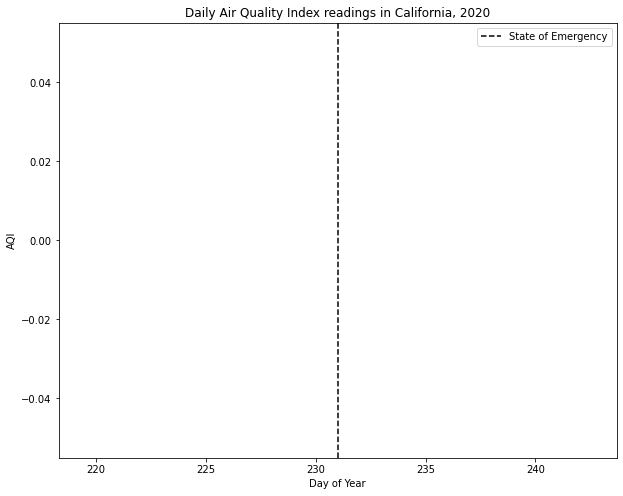
\includegraphics{W03. Spatial Data_files/figure-pdf/cell-15-output-2.png}

}

\end{figure}

We can see that the worst affected county suffered a massive spike in
AQI following the wildfires, while the least affected county experienced
a much smaller increase in AQI.

\hypertarget{bringing-in-geography}{%
\section{Bringing in Geography}\label{bringing-in-geography}}

We can explore some limited geographic variation using the ``COUNTY''
column in our dataframe. But we actually have the latitude and longitude
of each individual sensor. We can visualize latitude and longitude data
quite simply as a scatterplot.

Remember, in our original dataframe each row is a reading from a given
sensor on a given day. The sensor's location does not vary over time, so
if we simply plot our original dataframe, we'll have loads of points on
top of each other. Let's pick a specific date, take a slice of our
dataframe on that one date, and plot it. I've picked September 9th based
on the plots above (looks like air quality was really bad).

\begin{Shaded}
\begin{Highlighting}[]
\CommentTok{\# create a variable with the date of interest, September 9th 2020. }
\NormalTok{date}\OperatorTok{=}\StringTok{\textquotesingle{}09{-}09{-}2020\textquotesingle{}}

\CommentTok{\# filter the original dataframe using this date}
\NormalTok{one\_day}\OperatorTok{=}\NormalTok{df[df[}\StringTok{\textquotesingle{}Date\textquotesingle{}}\NormalTok{]}\OperatorTok{==}\NormalTok{date]}

\CommentTok{\# create a scatterplot of sensor locations using latitude and longitude }
\NormalTok{plt.scatter(}
\NormalTok{    x}\OperatorTok{=}\NormalTok{one\_day[}\StringTok{\textquotesingle{}longitude\textquotesingle{}}\NormalTok{],}
\NormalTok{    y}\OperatorTok{=}\NormalTok{one\_day[}\StringTok{\textquotesingle{}latitude\textquotesingle{}}\NormalTok{])}

\CommentTok{\# as always, label our axes and the plot!}
\NormalTok{plt.xlabel(}\StringTok{"Longitude"}\NormalTok{)}
\NormalTok{plt.ylabel(}\StringTok{"Latitude"}\NormalTok{)}
\NormalTok{plt.title(}\StringTok{"Geographic Distribution of AQI sensors in California"}\NormalTok{)}
\end{Highlighting}
\end{Shaded}

\begin{verbatim}
Text(0.5, 1.0, 'Geographic Distribution of AQI sensors in California')
\end{verbatim}

\begin{figure}[H]

{\centering 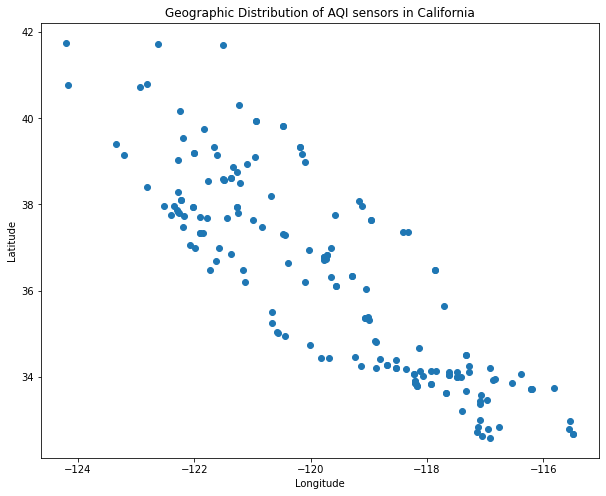
\includegraphics{W03. Spatial Data_files/figure-pdf/cell-16-output-2.png}

}

\end{figure}

If you close your eyes and imagine the shape of California, you can
probably see its outline roughly traced in the points above. This plot
leaves a number of things to be desired.

\hypertarget{basemaps}{%
\subsection{Basemaps}\label{basemaps}}

First, we may want to add in a base map of some kind so we can have a
better sense of where each sensor is. For this, we have to import an
extra library called ``Basemap''

\begin{Shaded}
\begin{Highlighting}[]
\CommentTok{\# import Basemap library}
\ImportTok{from}\NormalTok{ mpl\_toolkits.basemap }\ImportTok{import}\NormalTok{ Basemap}

\CommentTok{\# create a basemap, call it \textquotesingle{}map\textquotesingle{}}
\BuiltInTok{map} \OperatorTok{=}\NormalTok{ Basemap(projection}\OperatorTok{=}\StringTok{\textquotesingle{}lcc\textquotesingle{}}\NormalTok{, resolution}\OperatorTok{=}\StringTok{\textquotesingle{}l\textquotesingle{}}\NormalTok{, }\CommentTok{\# this selects the projection of the map.}
\NormalTok{            lat\_0}\OperatorTok{=}\FloatTok{37.5}\NormalTok{, lon\_0}\OperatorTok{={-}}\DecValTok{119}\NormalTok{, }\CommentTok{\# this sets the center of the map }
\NormalTok{            width}\OperatorTok{=}\FloatTok{1E6}\NormalTok{, height}\OperatorTok{=}\FloatTok{1.2E6}\NormalTok{) }\CommentTok{\# this sets the window that we\textquotesingle{}re looking at, in meters.}

\CommentTok{\# We can add features to our blank basemap, including coastlines, as well as state and country boundaries. }
\BuiltInTok{map}\NormalTok{.drawcoastlines(color}\OperatorTok{=}\StringTok{\textquotesingle{}black\textquotesingle{}}\NormalTok{)}
\BuiltInTok{map}\NormalTok{.drawcountries(color}\OperatorTok{=}\StringTok{\textquotesingle{}black\textquotesingle{}}\NormalTok{)}
\BuiltInTok{map}\NormalTok{.drawstates(color}\OperatorTok{=}\StringTok{\textquotesingle{}gray\textquotesingle{}}\NormalTok{)}

\CommentTok{\# Finally, we add in our AQI sensor data on top of the basemap.}
\BuiltInTok{map}\NormalTok{.scatter(}
\NormalTok{    one\_day[}\StringTok{\textquotesingle{}longitude\textquotesingle{}}\NormalTok{], }
\NormalTok{    one\_day[}\StringTok{\textquotesingle{}latitude\textquotesingle{}}\NormalTok{], }
\NormalTok{    latlon}\OperatorTok{=}\VariableTok{True}\NormalTok{)}

\CommentTok{\# as always, title your figure}
\NormalTok{plt.title(}\StringTok{"Geographic Distribution of AQI sensors in California"}\NormalTok{)}
\end{Highlighting}
\end{Shaded}

\begin{verbatim}
Text(0.5, 1.0, 'Geographic Distribution of AQI sensors in California')
\end{verbatim}

\begin{figure}[H]

{\centering 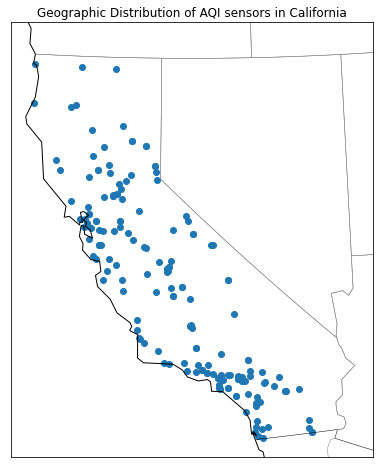
\includegraphics{W03. Spatial Data_files/figure-pdf/cell-17-output-2.png}

}

\end{figure}

That's looking a bit better! We now have a much better sense of the
actual distribution of these sensors within california. People who know
the area will recognize clusters of sensors around San Francisco and Los
Angeles; This makes sense, given that these areas have a higher
population density. However, our plot is still missing some pretty
important information: the actual AQI readings!

\hypertarget{colormaps}{%
\subsection{Colormaps}\label{colormaps}}

The whole point of plotting these sensors is to understand the spatial
distribution of air pollution from the 2020 wildfires.

The EPA published the following
\href{https://www.airnow.gov/aqi/aqi-basics/}{table} on their website,
which creates a color-coded scale of AQI values that corresponds to the
impact thereof on human health.

\begin{itemize}
\tightlist
\item
  AQI under 50 is colored green, and indicates ``Good'' air quality.
\item
  AQI between 100 and 200 is generally unhealthy
\item
  AQI over 300 is deemed hazardous.
\end{itemize}

With this in mind, quickly scroll back up to the AQI plots over time. If
you did everything correctly, you should notice that the \emph{average}
AQI value across all sensors in the worst affected county was over 600!

We'll be using the table from the EPA website to build our own color
map. In the code below, I scrape the table and turn it into a
``colormap'' (basically, a dictionary that associates numbers with
colors) that we'll use to color the AQI sensors later.

\begin{Shaded}
\begin{Highlighting}[]
\CommentTok{\# scrape the table of AQI values and corresponding colors }
\CommentTok{\# save it as a dataframe called colors}
\NormalTok{colors}\OperatorTok{=}\NormalTok{pd.read\_html(}\StringTok{\textquotesingle{}https://www.airnow.gov/aqi/aqi{-}basics/\textquotesingle{}}\NormalTok{)[}\DecValTok{0}\NormalTok{]}

\CommentTok{\# create a numerical column for AQI values by splitting the test in the "values of index" column. }
\CommentTok{\# pull out the first string, and convert it to integer}
\NormalTok{colors[}\StringTok{\textquotesingle{}aqi\textquotesingle{}}\NormalTok{]}\OperatorTok{=}\NormalTok{colors[}\StringTok{\textquotesingle{}Values of Index\textquotesingle{}}\NormalTok{].}\BuiltInTok{str}\NormalTok{.split(}\StringTok{\textquotesingle{} \textquotesingle{}}\NormalTok{).}\BuiltInTok{str}\NormalTok{[}\DecValTok{0}\NormalTok{].astype(}\BuiltInTok{int}\NormalTok{)}

\CommentTok{\# print three columns from the dataframe }
\BuiltInTok{print}\NormalTok{(colors[[}\StringTok{\textquotesingle{}aqi\textquotesingle{}}\NormalTok{,}\StringTok{\textquotesingle{}Daily AQI Color\textquotesingle{}}\NormalTok{,}\StringTok{\textquotesingle{}Levels of Concern\textquotesingle{}}\NormalTok{]])}

\CommentTok{\# create a "colormap" from this dataframe using the "Daily AQI Color" column, and the "aqi" column }
\NormalTok{aqi\_colors}\OperatorTok{=}\NormalTok{matplotlib.colors.LinearSegmentedColormap.from\_list(colors[}\StringTok{\textquotesingle{}aqi\textquotesingle{}}\NormalTok{],colors[}\StringTok{\textquotesingle{}Daily AQI Color\textquotesingle{}}\NormalTok{])}
\end{Highlighting}
\end{Shaded}

\begin{verbatim}
   aqi Daily AQI Color               Levels of Concern
0    0           Green                            Good
1   51          Yellow                        Moderate
2  101          Orange  Unhealthy for Sensitive Groups
3  151             Red                       Unhealthy
4  201          Purple                  Very Unhealthy
5  301          Maroon                       Hazardous
\end{verbatim}

Now, we can use this ``aqi\_colors'' object as a color palette later
when we plot the AQI sensors. This way, we will know that green and
yellow points are OK, while red and purple points represent hazardous
levels of air pollution. I've annotated the code above, but it's ok if
you don't get all of it. You could simply load a different colormap in
one line of code; check out the documentation
\href{https://matplotlib.org/stable/tutorials/colors/colormaps.html}{here}.

\begin{Shaded}
\begin{Highlighting}[]
\BuiltInTok{map} \OperatorTok{=}\NormalTok{ Basemap(projection}\OperatorTok{=}\StringTok{\textquotesingle{}lcc\textquotesingle{}}\NormalTok{, resolution}\OperatorTok{=}\StringTok{\textquotesingle{}l\textquotesingle{}}\NormalTok{, }
\NormalTok{            lat\_0}\OperatorTok{=}\FloatTok{37.5}\NormalTok{, lon\_0}\OperatorTok{={-}}\DecValTok{119}\NormalTok{,}
\NormalTok{            width}\OperatorTok{=}\FloatTok{1E6}\NormalTok{, height}\OperatorTok{=}\FloatTok{1.2E6}\NormalTok{)}

\BuiltInTok{map}\NormalTok{.drawcoastlines(color}\OperatorTok{=}\StringTok{\textquotesingle{}black\textquotesingle{}}\NormalTok{)}
\BuiltInTok{map}\NormalTok{.drawcountries(color}\OperatorTok{=}\StringTok{\textquotesingle{}black\textquotesingle{}}\NormalTok{)}
\BuiltInTok{map}\NormalTok{.drawstates(color}\OperatorTok{=}\StringTok{\textquotesingle{}gray\textquotesingle{}}\NormalTok{)}

\BuiltInTok{map}\NormalTok{.scatter(}
\NormalTok{      one\_day[}\StringTok{\textquotesingle{}longitude\textquotesingle{}}\NormalTok{], }
\NormalTok{      one\_day[}\StringTok{\textquotesingle{}latitude\textquotesingle{}}\NormalTok{], }
\NormalTok{      latlon}\OperatorTok{=}\VariableTok{True}\NormalTok{, }
\NormalTok{      c}\OperatorTok{=}\NormalTok{one\_day[}\StringTok{\textquotesingle{}AQI\textquotesingle{}}\NormalTok{], }\CommentTok{\# We\textquotesingle{}re adding that }
\NormalTok{      cmap}\OperatorTok{=}\NormalTok{aqi\_colors, }
\NormalTok{      vmin}\OperatorTok{=}\DecValTok{0}\NormalTok{, }
\NormalTok{      vmax}\OperatorTok{=}\DecValTok{300}\NormalTok{)}


\NormalTok{plt.title(}\StringTok{\textquotesingle{}Air Quality on September 9th, 2020\textquotesingle{}}\NormalTok{)}
\NormalTok{plt.colorbar(label}\OperatorTok{=}\StringTok{\textquotesingle{}Air Quality Index\textquotesingle{}}\NormalTok{)}\OperatorTok{;}
\end{Highlighting}
\end{Shaded}

\begin{figure}[H]

{\centering 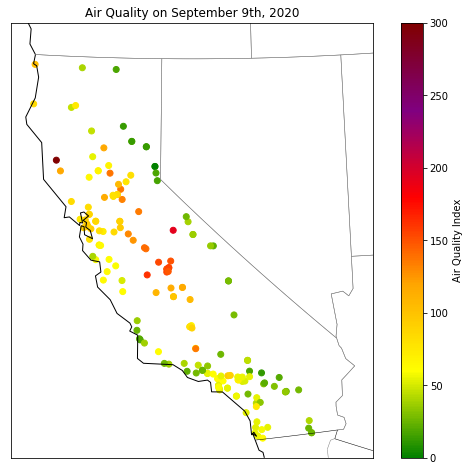
\includegraphics{W03. Spatial Data_files/figure-pdf/cell-19-output-1.png}

}

\end{figure}

This plot gives us a good sense of which areas were worst affected by
the wildfires on September 9th, 2020. Areas in the central valley
suffered particularly bad air quality, with AQI reaching hazardous
levels in some areas.

\hypertarget{exercise-3}{%
\subsection{Exercise}\label{exercise-3}}

So far, we've been plotting data from one day, using a dataframe we
generated by filtering the date column like so:
\texttt{one\_day=df{[}df{[}\textquotesingle{}Date\textquotesingle{}{]}==\textquotesingle{}09-09-2020\textquotesingle{}{]}}
(date format is day-month-year).

Using the code from the previous cell, generate a plot of AQI on March
2nd, 2020. After that, use the groupby function to generate a plot of
the maximum AQI reading for each sensor and plot it.

If you've followed along this far, well done! we've come a long way from
a spreadsheet full of sensor readings. But we can go even further!

\hypertarget{advanced-satellite-imagery-and-interactivity}{%
\section{Advanced: Satellite Imagery and
Interactivity}\label{advanced-satellite-imagery-and-interactivity}}

The AQI plots we've generated above give us a good sense of where the
worst air pollution was on a given day; but we're still basically
\emph{inferring} the presence of fires. Luckily, we don't have to do
that. The plumes of smoke generated by the fires were so vast that they
were visible from space. There are a variety of satellites that image
the earth each day (some, like GOES-17, take a picture every few
minutes!).

NASA's Moderate Resolution Imaging Spectroradiometer (MODIS) satellites
take a picture of the same spot on earth nearly every day. So far, we've
been looking at September 9th as a particularly bad day for air quality
in California. Let's have a look at a satellite image from that day. A
Python library called ipyleaflet contains some useful functions that let
us pull up an interactive map of satellite imagery.

\begin{Shaded}
\begin{Highlighting}[]
\CommentTok{\# import the map making modules from ipyleaflet}
\ImportTok{from}\NormalTok{ ipyleaflet }\ImportTok{import}\NormalTok{ Map, Marker, basemaps, basemap\_to\_tiles,Circle}

\CommentTok{\# let create an interactive Map object called "satellite\_map"}
\NormalTok{satellite\_map }\OperatorTok{=}\NormalTok{ Map(}
\NormalTok{  basemap}\OperatorTok{=}\NormalTok{basemap\_to\_tiles( }\CommentTok{\#this function lets us pick from a list of basemaps for our interactive map}
\NormalTok{    basemaps.NASAGIBS.ModisTerraTrueColorCR, }\StringTok{"2020{-}09{-}09"} \CommentTok{\# here we\textquotesingle{}re specifying that we want MODIS imagery, and the date that we want it from  }
\NormalTok{  ),}
\NormalTok{  center}\OperatorTok{=}\NormalTok{(}\FloatTok{36.77}\NormalTok{, }\OperatorTok{{-}}\FloatTok{119.41}\NormalTok{), }\CommentTok{\# then, we want to center the map on california. these coordinates do that}
\NormalTok{  zoom}\OperatorTok{=}\DecValTok{5}\NormalTok{, }\CommentTok{\#finally, we want to set the zoom level of the map. }
\NormalTok{)}

\CommentTok{\# once we\textquotesingle{}ve created the map object we can make it bigger or smaller. let\textquotesingle{}s make it 700 pixels tall. }
\NormalTok{satellite\_map.layout.height }\OperatorTok{=} \StringTok{\textquotesingle{}700px\textquotesingle{}}

\CommentTok{\# now, we visualize it.}
\NormalTok{satellite\_map}
\end{Highlighting}
\end{Shaded}

\begin{verbatim}
Map(center=[36.77, -119.41], controls=(ZoomControl(options=['position', 'zoom_in_text', 'zoom_in_title', 'zoom…
\end{verbatim}

This is a pretty striking image of the West Coast of the U.S. We can see
fluffy white clouds to the East and West, but in the center of the map
plumes of brown smoke emanate from wildfires in California and Oregon.
Use the + - keys in the top left to zoom in, see if you can spot some
wildfires.

\hypertarget{exercise-4}{%
\subsection{Exercise}\label{exercise-4}}

Try changing the code in the cell above to display an image from
September 15th. You could even try importing a different basemap (like
nighttime lights) using this
\href{https://ipyleaflet.readthedocs.io/en/latest/map_and_basemaps/basemaps.html}{list
of basemaps}.

\hypertarget{combining-sensors-and-satellite-images}{%
\section{Combining sensors and satellite
images}\label{combining-sensors-and-satellite-images}}

A cool part of working with spatial data is that we can combine two
completeley different datasets using spatial information. We can add the
AQI sensor data as points to this map.

\begin{Shaded}
\begin{Highlighting}[]
\CommentTok{\# grab the first row from our September 9th dataframe}
\NormalTok{row}\OperatorTok{=}\NormalTok{one\_day.iloc[}\DecValTok{0}\NormalTok{]}
\BuiltInTok{print}\NormalTok{(row)}

\CommentTok{\# This part uses the AQI value in this row (72), and looks up the corresponding color in the colormap we created earlier }
\NormalTok{color}\OperatorTok{=}\NormalTok{matplotlib.colors.rgb2hex(aqi\_colors(row[}\StringTok{\textquotesingle{}AQI\textquotesingle{}}\NormalTok{]))}

\CommentTok{\# Now we create a Circle object using the latitude and longitude from the row, and color it using the color we just selected}
\NormalTok{point}\OperatorTok{=}\NormalTok{Circle(location}\OperatorTok{=}\NormalTok{(row[}\StringTok{\textquotesingle{}latitude\textquotesingle{}}\NormalTok{],row[}\StringTok{\textquotesingle{}longitude\textquotesingle{}}\NormalTok{]), color}\OperatorTok{=}\NormalTok{color)}

\CommentTok{\# Add this as a layer to the satellite\_map object}
\NormalTok{satellite\_map.add\_layer(point)}

\CommentTok{\# Display the updated map}
\NormalTok{satellite\_map}
\end{Highlighting}
\end{Shaded}

\begin{verbatim}
Date                       2020-09-09 00:00:00
Site ID                               60010007
POC                                          3
PM                                        22.3
AQI                                         72
Site Name                            Livermore
CBSA_NAME    San Francisco-Oakland-Hayward, CA
COUNTY                                 Alameda
latitude                             37.687526
longitude                          -121.784217
Month                                        9
Day                                        253
Name: 249, dtype: object
\end{verbatim}

\begin{verbatim}
Map(center=[36.77, -119.41], controls=(ZoomControl(options=['position', 'zoom_in_text', 'zoom_in_title', 'zoom…
\end{verbatim}

It's a bit hard to see, but we've plotted an AQI sensor! its under the
cloud of smoke in the center of the map. You can zoom in to get a closer
look. looks like AQI was pretty bad at this location.

Having plotted one point, we can now plot all the points on September
9th! to do so, we can use the \texttt{iterrows} function in Pandas
which, suprisingly, lets you iterate over rows in a dataframe. The first
line of code below allows us to iterate over the rows in the
\texttt{one\_day} dataframe. It will then run everything in the indented
block for each row; in other words, for each row, it will:

\begin{enumerate}
\def\labelenumi{\arabic{enumi}.}
\tightlist
\item
  use the row's value in the AQI value to select a color for the point
\item
  create a point object using the latitude and longitude columns
\item
  add that point to the satellite map.
\end{enumerate}

\begin{Shaded}
\begin{Highlighting}[]
\ControlFlowTok{for}\NormalTok{ index, row }\KeywordTok{in}\NormalTok{ one\_day.iterrows():}
\NormalTok{  color}\OperatorTok{=}\NormalTok{matplotlib.colors.rgb2hex(aqi\_colors(row[}\StringTok{\textquotesingle{}AQI\textquotesingle{}}\NormalTok{]))}
\NormalTok{  point}\OperatorTok{=}\NormalTok{Circle(location}\OperatorTok{=}\NormalTok{(row[}\StringTok{\textquotesingle{}latitude\textquotesingle{}}\NormalTok{],row[}\StringTok{\textquotesingle{}longitude\textquotesingle{}}\NormalTok{]), color}\OperatorTok{=}\NormalTok{color)}
\NormalTok{  satellite\_map.add\_layer(point)}

\CommentTok{\# display the map}
\NormalTok{satellite\_map}
\end{Highlighting}
\end{Shaded}

\begin{verbatim}
Map(center=[36.77, -119.41], controls=(ZoomControl(options=['position', 'zoom_in_text', 'zoom_in_title', 'zoom…
\end{verbatim}

Theres a pretty striking trend in this data. If you zoom in, you'll see
that the AQI sensors to the East are all green since they are up-wind
from the fires. A few kilometers downwind of the fires, the AQI sensors
display very high readings. Remember, our AQI data and the satellite
imagery are derived from totally different sources, and are totally
different types of data, but they seem to be telling us the same story.
They actually complement each other in important ways. In our original
plot of the AQI sensors without satellite imagery, we could tell that
there was bad air quality on September 9th, but some sensors were green
and others were red. The satellite image shows us that the variation in
AQI across California on September 9th was due to the direction of the
wind, blowing the smoke from the wildfires westward.

\hypertarget{extension}{%
\section{Extension}\label{extension}}

Now, to save some hassle we can package all the code we used to generate
this map into one clean function. Because we're effectively just
changing the date, we can configure this function so that we can feed it
a different date, and it will grab a satellite image and filter our
dataframe for values occuring on that day. Then, we can draw a new map
in one line of code.

\begin{Shaded}
\begin{Highlighting}[]
\KeywordTok{def}\NormalTok{ satellite\_plot(date):}
  
\NormalTok{  ymd}\OperatorTok{=}\NormalTok{datetime.strptime(date, }\StringTok{\textquotesingle{}}\SpecialCharTok{\%d}\StringTok{{-}\%m{-}\%Y\textquotesingle{}}\NormalTok{).strftime(}\StringTok{\textquotesingle{}\%Y{-}\%m{-}}\SpecialCharTok{\%d}\StringTok{\textquotesingle{}}\NormalTok{)}

\NormalTok{  satellite\_map }\OperatorTok{=}\NormalTok{ Map(}
\NormalTok{    basemap}\OperatorTok{=}\NormalTok{basemap\_to\_tiles(}
\NormalTok{      basemaps.NASAGIBS.ModisTerraTrueColorCR, ymd}
\NormalTok{    ),}
\NormalTok{    center}\OperatorTok{=}\NormalTok{(}\FloatTok{36.77}\NormalTok{, }\OperatorTok{{-}}\FloatTok{119.41}\NormalTok{),}
\NormalTok{    zoom}\OperatorTok{=}\DecValTok{6}\NormalTok{,}
\NormalTok{  )}

\NormalTok{  satellite\_map.layout.height }\OperatorTok{=} \StringTok{\textquotesingle{}700px\textquotesingle{}}

\NormalTok{  one\_day}\OperatorTok{=}\NormalTok{df[df[}\StringTok{\textquotesingle{}Date\textquotesingle{}}\NormalTok{]}\OperatorTok{==}\NormalTok{date]}

  \ControlFlowTok{for}\NormalTok{ index, row }\KeywordTok{in}\NormalTok{ one\_day.iterrows():}
\NormalTok{    color}\OperatorTok{=}\NormalTok{matplotlib.colors.rgb2hex(aqi\_colors(row[}\StringTok{\textquotesingle{}AQI\textquotesingle{}}\NormalTok{]))}
\NormalTok{    point}\OperatorTok{=}\NormalTok{Circle(location}\OperatorTok{=}\NormalTok{(row[}\StringTok{\textquotesingle{}latitude\textquotesingle{}}\NormalTok{],row[}\StringTok{\textquotesingle{}longitude\textquotesingle{}}\NormalTok{]), color}\OperatorTok{=}\NormalTok{color)}
\NormalTok{    satellite\_map.add\_layer(point)}
  \ControlFlowTok{return}\NormalTok{ satellite\_map}

\end{Highlighting}
\end{Shaded}

Now, we can simply change the date in the function and view both
satellite imagery and AQI sensor data from a given day. Look at this
clear day from February 3rd.

\begin{Shaded}
\begin{Highlighting}[]
\NormalTok{satellite\_plot(}\StringTok{\textquotesingle{}02{-}03{-}2020\textquotesingle{}}\NormalTok{)}
\end{Highlighting}
\end{Shaded}

\begin{verbatim}
Map(center=[36.77, -119.41], controls=(ZoomControl(options=['position', 'zoom_in_text', 'zoom_in_title', 'zoom…
\end{verbatim}

All the AQI sensors are showing green values, indicating generally good
air quality. The satellite image shows a few wispy clouds, but no thick
yellow smoke. Now change the date to September 15th, and see what
happens!



\end{document}
